In this section, we first introduce the neural architecture of \our in Section~\ref{section:method_details} then explicitly highlight its difference to baseline methods in Section~\ref{section:some_differences}.

\subsection{Details on \oure: neural architecture and input data} \label{section:method_details}

\our has three modules: \circled{1} \emph{link-encoder} is designed to summarize the information from temporal links (e.g., link timestamps and link features); \circled{2} \emph{node-encoder} is designed to summarize the information from nodes (e.g., node features and node identity); \circled{3} \emph{link classifier} predicts whether a link exists based on the output of the aforementioned two encoders.

\noindent\textbf{Link-encoder.}
The link-encoder is designed to summarize the temporal link information associated with each node sorted by timestamps, where temporal link information is referring to the timestamp and features of each link.
For example in Figure~\ref{fig:temporal_graph_with_feats}, the temporal link information for node $v_2$  is \smash{$\{ (t_1, \mathbf{x}_{1,2}^\text{link}(t_1)), (t_3, \mathbf{x}_{2,4}^\text{link}(t_3)), (t_4, \mathbf{x}_{2,4}^\text{link}(t_4)), (t_5, \mathbf{x}_{1,2}^\text{link}(t_5)) \}$} and for node $v_5$ is \smash{$\{ (t_2, \mathbf{x}_{3,5}^\text{link}(t_2)), (t_6, \mathbf{x}_{4,5}^\text{link}(t_6))\}$}.
% If the temporal graph is undirected and two nodes frequently interact with each other recently, they are expected to have similar temporal link information.
% Intuitively, two nodes are likely to be linked in the near future if they are frequently connected by links in the last few timestamps.
In practice, we only keep the top $K$ most recent temporal link information, where $K$ is a dataset dependent hyper-parameter.
If multiple links have the same timestamps, we simply keep them the same order as the input raw data.
To summarize temporal link information, our link-encoder should have the ability to distinguish different timestamps (achieved by our time-encoding function) and different temporal link information (achieved by the Mixer module).
\begin{itemize} [noitemsep,topsep=0pt,leftmargin=5mm ]
    \item \textit{Time-encoding function.} To distinguish different timestamps, we introduce our time-encoding function $\cos(t\boldsymbol{\omega})$, which utilizes features \smash{$\boldsymbol{\omega} = \{ \alpha^{-(i-1)/\beta} \}_{i=1}^{d}$} to encode each timestamps into a $d$-dimensional vector. 
    More specifically, we first map each $t$ to a vector with monotonically exponentially decreasing values $t\boldsymbol{\omega} \in (0, t]$ among the feature dimension, then use cosine function to project all values to $\cos(t\boldsymbol{\omega}) \in [-1,+1]$.
    The selection of $\alpha,\beta$ is depending on the scale of the maximum timestamp $t_{\max}$ we wish to encode. In order to distinguish all timestamps, we have to make sure \smash{$t_{\max} \times \alpha^{-(i-1)/\beta} \rightarrow 0$} as $i\rightarrow d$ to distinguish all timestamps.
    In practice, we found $d=100$ and \smash{$\alpha=\beta=\sqrt{d}$} works well for all datasets. 
    Notice that $\boldsymbol{\omega}$ is fixed and will not be updated during training.
    As shown in Figure~\ref{fig:temporal_encoder}a,
    the output of this time-encoding function has two main properties that could help \our distinguish different timestamps: similar timestamps have similar time-encodings (e.g., the plot of $t_1,t_2$) and the larger the timestamp the later the values in time-encodings converge to $+1$ (e.g., the plot of $t_1,t_3$ or $t_1, t_4$).
    \item \textit{Mixer for information summarizing.} We use a 1-layer MLP-mixer~\cite{tolstikhin2021mlp} to summarize the temporal link information. Figure~\ref{fig:temporal_encoder}b is an example on summarizing the temporal link information of node $v_2$. Recall that the temporal link information of node $v_2$  is $\{ (t_1, \mathbf{x}_{1,2}^\text{link}(t_1)), (t_3, \mathbf{x}_{2,4}^\text{link}(t_3)), (t_4, \mathbf{x}_{2,4}^\text{link}(t_4)), (t_5, \mathbf{x}_{1,2}^\text{link}(t_5)) \}$. We first encode timestamps by our time-encoding function then concatenate it with its corresponding link features. For example, we encode \smash{$(t_1, \mathbf{x}_{1,2}^\text{link}(t_1))$} as \smash{$[\cos((t_0-t_1)\boldsymbol{\omega})~||~\mathbf{x}_{1,2}^\text{link}(t_1))]$} where $t_0$ is the timestamp that we want to predict whether the link exists. Then, we stack all the outputs into a big matrix and zero-pad to the fixed length $K$ denoted as $\mathbf{T}_2(t_0)$.
    Finally, we use an 1-layer MLP-mixer with mean-pooling to compress $\mathbf{T}_2(t_0)$ into a single vector $\mathbf{t}_2(t_0)$.
    Specifically, the MLP-mixer takes $\mathbf{T}_2(t_0)$  as input
    \begin{equation*} % \label{eq:mlp_mixer}
        \begin{aligned}
        \mathbf{T}_2(t_0)\rightarrow \mathbf{H}_\text{input},~ \mathbf{H}_\text{token} &= \mathbf{H}_\text{input} + \mathbf{W}_\text{token}^{(2)} \texttt{GeLU}(\mathbf{W}_\text{token}^{(1)} \texttt{LayerNorm}(\mathbf{H}_\text{input})),\\
        \mathbf{H}_\text{channel} &= \mathbf{H}_\text{token} +  \texttt{GeLU}( \texttt{LayerNorm}(\mathbf{H}_\text{token})\mathbf{W}_\text{channel}^{(1)} ) \mathbf{W}_\text{channel}^{(2)},\\
        \end{aligned}
    \end{equation*}
     and output the temporal encoding \smash{$\mathbf{t}_2(t_0)= \texttt{Mean}(\mathbf{H}_\text{channel})$}.
    Please notice that zero-padding operator is important to capture how often a node interacts with other nodes. The node with more zero-padded dimensions has less temporal linked neighbors. This information is very important in practice according to our experimental observation.
\end{itemize}


\begin{figure}[t]
    \centering
    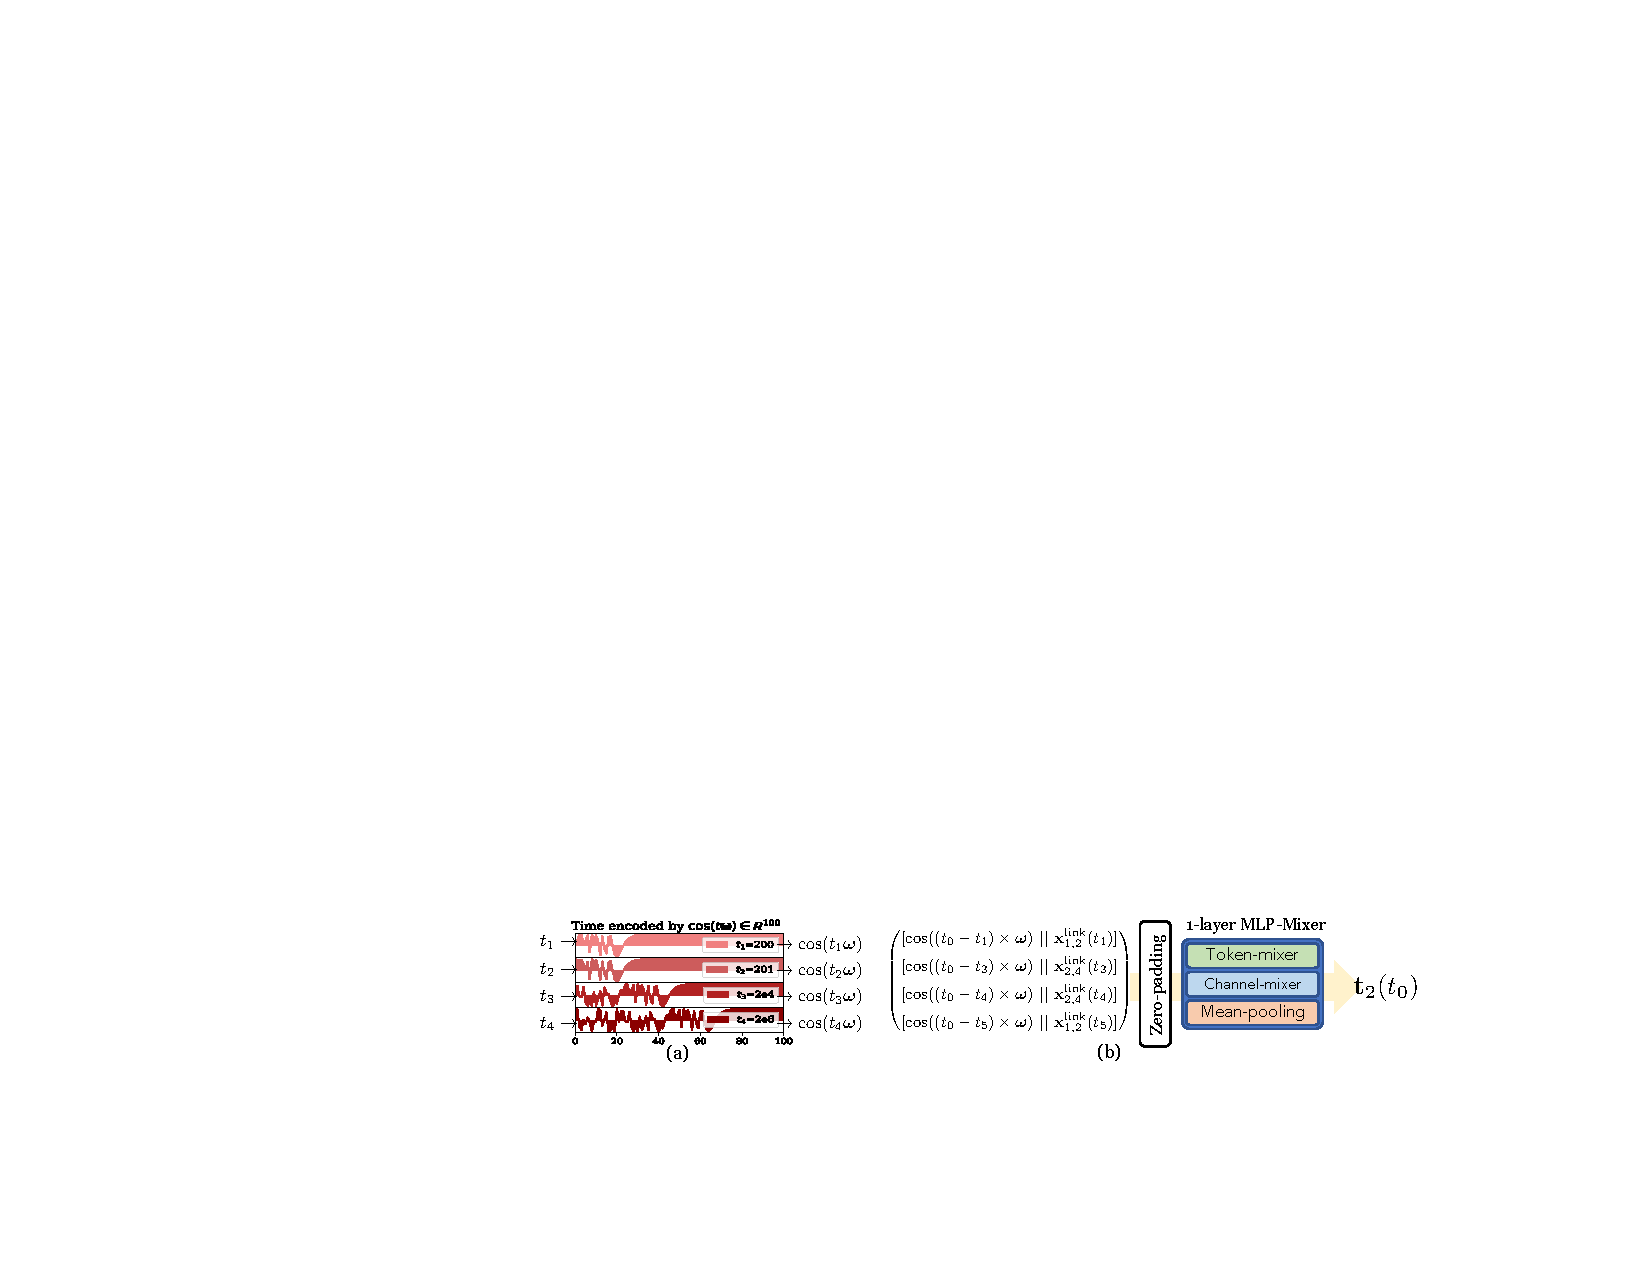
\includegraphics[width=0.99\textwidth]{figures/temporal_encoder.pdf}
    \vspace{-4mm}
    \caption{(a) Time-encoding function that pre-process timestamp $t$ into a vector $\cos(t\boldsymbol{\omega})$. The x-axis is the vector dimension and the y-axis is the cosine value. (b) link-encoder takes the temporal link information of node $v_2$ as inputs and outputs a vector $\mathbf{t}_2(t_0)$ that will be used for link prediction.}
    \label{fig:temporal_encoder}
    \vspace{-3mm}
\end{figure}

\noindent\textbf{Node-encoder.}
The node-encoder is designed to capture the node identity and node feature information via neighbor mean-pooling.
% Intuitively, two nodes are more likely to have interaction if they both interact with some other nodes recently.
Let us define the 1-hop neighbor of node $v_i$ with link timestamps from $t$ to $t_0$ as $\mathcal{N}(v_i; t, t_0)$. 
For example in Figure~\ref{fig:temporal_graph_with_feats}, we have $\mathcal{N}(v_2; t_4, t_0) = \{v_1, v_4\}$ and $\mathcal{N}(v_5; t_4, t_0) = \{v_3\}$. 
Then, the node-info feature is computed based on the 1-hop neighbor by 
\smash{$\mathbf{s}_i(t_0) = \mathbf{x}_i^\text{node} + \texttt{Mean}\{\mathbf{x}_j^\text{node}~|~v_j\in \mathcal{N}(v_i; t_0-T, t_0) \}$}, where $T$ is a dataset-dependent hyper-parameter.
In practice, we found 1-hop neighbors are enough to achieve good performance, and we use one-hot node representations for datasets without node features.


\noindent\textbf{Link classifier.} 
Link classifier is designed to classify whether a link exists at time $t_0$ using the output of link-encoder $\mathbf{t}_i(t_0)$ and the output of node-encoder $\mathbf{s}_i(t_0)$.
Let us denote the node $v_i$'s representation at time $t_0$ as the concatenation of the above two encodings $\mathbf{h}_i(t_0) = [\mathbf{s}_i(t_0)~||~\mathbf{t}_i(t_0)]$.
Then, the prediction on whether an interaction between node $v_i,v_j$ happens at time $t_0$ is computed by applying a 2-layer MLP model on $[\mathbf{h}_i(t_0)~||~\mathbf{h}_j(t_0)]$, i.e., $p_{ij} = \texttt{MLP}([\mathbf{h}_i(t_0)~||~\mathbf{h}_j(t_0)])$.
% We share the same link prediction classifier with baselines. 

\subsection{Comparison to existing methods} \label{section:some_differences}

In the following, we highlight some differences between \our and other methods, which will be explicitly ablation studied in the experiment section (Section~\ref{section:data_alignment}). 

\noindent\textbf{Temporal graph as undirected graph.}
Most of the existing works consider temporal graphs as directed graphs with information only flows from the source node (e.g., users in the recommender system) to the destination nodes (e.g., ads in the recommender system). However, we consider the temporal graph as an undirected graph.
By doing so, if two nodes are frequently connected in the last few timestamps, the ``most recent 1-hop neighbors'' sampled for the two nodes on the ``undirected'' temporal graph would be similar.
In other words, the similarity between the sampled neighbors provides information on whether two nodes are frequently connected in the last few timestamps, which is essential for temporal graph link prediction. Intuitively, if two nodes are frequently connected in the last few timestamps, they are also likely to be connected in the recent future.

\noindent\textbf{Selection on neighbors.}
Existing methods consider either ``multi-hop recent neighbors'' or ``multi-hop uniform sampled neighbors'', whereas we only consider the ``$1$-hop most recent neighbors''. For example, TGAT~\cite{xu2020inductive}, DySAT~\cite{sankar2020dysat}, and TGSRe~\cite{fan2021continuous} consider multi-hop uniform sampled neighbors; JODIE~\cite{kumar2019predicting}, TGN~\cite{tgn_icml_grl2020}, and APAN~\cite{wang2021apan} maintain the historical node interactions via RNN, which can be think of as multi-hop recent neighbors; CAWs~\cite{wang2020inductive} samples neighbors by random walks, which can also be think of as multi-hop recent neighbors.
Although sampling more neighbors could provide a sufficient amount of information for models to reason about, it could also carry much spurious or noisy information. As a result, more complicated model architectures (e.g., RNN or SAM) are required to extract useful information from the raw data, which could lead to a poor model trainability and potentially weaker generalization ability.  
Instead, we only take the ``most recent 1-hop neighbors'' into consideration, which is conceptually simpler and enjoys better performance. 


% \subsection{Simpler model generalization better}

% One of the major factors that contribute to the success of \our is the simplicity of \oure's neural architecture and the selection of input data.
% Selecting input data that better aligned with their labels allows a simple neural network model is enough to capture the underlying mapping between the input to their labels, which could lead to a better generalization ability than a complex neural network model.

% In the following, we rigorously formulate the above arguments by analyzing the generalization ability of a model. Our result assumes that the training and evaluation data have different sampling distribution, which is the same case in temporal graph link prediction because the underlying data distribution evolves over time.
% For any given node $v_i$,
% let us recall that $\mathbf{T}_i(t_0)$ is the input of link-encoder and $\mathbf{s}_i(t_0)$ is the input of node-encoder. 
% For notation simplicity, let us define $\mathbf{x}_i = [\text{vec}(\mathbf{T}_i(t_0))~||~\mathbf{s}_i(t_0)]$ as the vectorized input of \our for node $v_i$ and define $\mathbf{x}_{ij} = [\mathbf{x}_i~||~\mathbf{x}_j]$ as the concatenation of $\mathbf{x}_i, \mathbf{x}_j$.
% For analysis purpose, we consider a more general case that the link between $v_i, v_j$ is predicted by applying a $L$-layer ReLU MLP model $f\in\mathcal{F}$ on the $\mathbf{x}_{ij}$, where $f$ is a $L$-layer MLP that is parameterized by \smash{$\boldsymbol{\theta} = \{\mathbf{W}^{(1)},\ldots,\mathbf{W}^{(L)}\}$.}
% Our goal is to upper bound the evaluation error \smash{$\mathcal{R}_\text{eval}(f)$} in Corollary~\ref{corollary:rademacher_bound}.
% The proof is deferred to Appendix~\ref{section:generalization}.

% \begin{corollary}\label{corollary:rademacher_bound}
% Let us define $\mathcal{D}_\text{train}$ as the training set sampled with distribution $P_\text{train}$ and $\mathcal{D}_\text{eval}$ as the evaluation set sampled with distribution $P_\text{eval}$. Let us assume the output of MLP is bounded $C = \sup_{\mathbf{x}\in\mathcal{X}} |f(\mathbf{x})|$.
% Let us define the evaluation error as $\mathcal{R}_\text{eval}(f) = \frac{1}{|\mathcal{D}_\text{eval}|} \sum_{(v_i, v_j)\in \mathcal{D}_\text{eval}} \mathbf{1}\{y_{ij} f(\mathbf{x}_{ij}) \leq 0\}$ and the  training error as $\mathcal{R}_\text{train}^\gamma(f) = \frac{1}{|\mathcal{D}_\text{train}|} \sum_{(v_i, v_j)\in \mathcal{D}_\text{train}} \mathbf{1}\{y_{ij} f(\mathbf{x}_{ij}) \leq \gamma\}$ for any $\gamma >0$. Then,
% with probability at least $1-\delta$, we can upper bound the evaluation error by
% \begin{equation*}
%     \mathcal{R}_\text{eval}(f) \leq \mathcal{R}_\text{train}^\gamma(f) + Q_{\gamma, \delta, C, |\mathcal{V}_\text{train}|} + \mathcal{O}\left( \frac{ \sqrt{D_{\chi^2}+1} \sqrt{L} B_X B_W^L }{\gamma \sqrt{|\mathcal{D}_\text{train}|}}\right) + D_{\ell_1},
% \end{equation*}
% where we have \smash{$B_X = \max_{i\neq j} \| \mathbf{x}_{ij} \|_2$} as the upper bound on the $\ell_2$-norm of input features, \smash{$B_W = \max\{1, \| \mathbf{W}^{(1)} \|_\mathrm{F}, \ldots, \|\mathbf{W}^{(L)} \|_\mathrm{F}\}$} as the upper bound on the Frobenius norm of weight parameters, \smash{$D_{\chi^2}=\int \left((d P_\text{train} / d P_\text{eval})^2 - 1 \right) d P_\text{eval}$} as the $\chi^2$-distance between $P_\text{train}$ and $P_\text{eval}$, \smash{$D_{\ell_1} = \frac{1}{n}\sum_{(v_i, v_j) \in \mathcal{D}_\text{train}} |P_\text{eval}(\mathbf{x}_{ij})/P_\text{train}(\mathbf{x}_{ij})-1|$} as the $\ell_1$-norm distance of two probability on the training set $\mathcal{D}_\text{train}$, and $Q_{\gamma,\delta,C,|\mathcal{V}_\text{train}|}$ is a constant that is related to $\gamma,\delta,C,|\mathcal{V}_\text{train}|$.
% \end{corollary}

% From Corollary~\ref{corollary:rademacher_bound}, we know the upper bound of the evaluation error $\mathcal{R}_\text{eval}$ is mainly affected by the training error $\mathcal{R}_\text{train}^\gamma$, the number of layers $L$, the discrepancy between training and evaluation distribution $D_{\chi^2},D_{\ell_1}$, and the number of training data $|\mathcal{D}_\text{train}|$. 

% In the following, we give several examples on how \our benefits from selecting good input data:
% \circled{1} In \oure, selecting input data that  better aligned to its label  allows us to use a simpler model to learn the underlying mapping between inputs to labels, without actually hurting the training error $\mathcal{R}_\text{train}^\gamma$ when switching to a simpler model architecture (i.e., a smaller number of layers $L$).
% For example, instead of feeding the raw timestamp to \our and encoding each timestamp with a trainable time-encoding function, \our pre-process the timestamps via our fixed time-encoding function and feed the pre-processed representation to \oure, which reduces the model complexity of learning a time-encoding function from data. 
% \circled{2} Selecting the input data that are less affected by the training and evaluation distribution deviation could also potentially improve the evaluation error. For example, using absolute timestamps (e.g., using Unix timestamp) is less preferred than using relative timestamps (i.e., each neighbor's timestamp is subtracted by its root node's timestamp) because the absolute timestamps in the evaluation set and training set are from different range when using chronological splits, but they are very likely to overlap if using relative timestamps.
% \circled{3} Selecting the most representative neighbors for each node. For example, we found 1-hop most recent interacted neighbors are the most representative for link prediction. Switching to either 2-hop neighbors or uniform sampled neighbors will hurt the model performance.



% \begin{remark}
% \weilin{
% According to our observation, selecting data that could explicitly capture the following information is essential for temporal graph link prediction: \circled{1} the ``most recent 1-hop neighbors'' sampled on the ``undirected'' temporal graph could give us information on whether two nodes are frequently connected in the last few timestamps; \circled{2} The ``relative time-gap of the root node to its neighbors'' and the ``number of neighbor nodes'' could give us information on how frequent a root node has interacted with other nodes.}
% \end{remark}

